\section{Matching and Vertex Covers}

\begin{definition}[Vertex Cover]
  A set \(U \subseteq V\) is a \textit{vertex cover} of \(E\) if
  every edge of \(G\) is incident with a vertex in \(U\).
\end{definition}

\begin{definition}[Edge Covers]
  An \textit{edge cover} of a graph \(G\) is a set of edges \(F
  \subseteq E(G)\) such that every vertex in \(G\) is 
  incident to an edge in \(F\).
\end{definition}

Intuitively, this means that the edge cover is a subgraph of edges that contains
every vertex in the original graph. Note that edge covers only exists for 
graphs with no isolated vertex since any isolated vertex would not be incident 
to any edge. Here are a few more numbers related to edge covers.

\begin{definition}[Edge Cover Number]
  The \textit{edge cover number} of a graph \(G\), denoted 
  \(\beta'(G)\), is the minimum size of an edge cover of \(G\).
\end{definition}

\begin{definition}[Edge Independence Number]
  The \textit{edge independence number}, denoted \(\alpha'(G)\),
  is the maximum size of any matching of \(G\). 
\end{definition}

\begin{definition}[Vertex Cover Number]
  The \textit{vertex cover number}, denoted \(\beta(G)\), is the
  minimum size of a vertex cover of \(G\).
\end{definition}

\begin{definition}[Vertex Independence Number]
  The \textit{vertex independence number}, denoted \(\alpha(G)\),
  is the maximum number of vertices of \(G\) such that no two of
  which are adjacent.
\end{definition}

\begin{table}[h]
  \centering
  \caption{Examples of edge cover-adjacent numbers}
  \begin{tabular}{|c|c|c|c|c|}
    \toprule
    Graph & \(\beta'(G)\) & \(\alpha'(G)\) & \(\beta(G)\) & \(\alpha(G)\) \\
    \midrule
    \(C_{n}\) with \(n\) even & \(n/2\) & \(n/2\) & \(2\) & \(n/2\) \\
    \(K_n\) with \(n\) even & \(n/2\) & \(n/2\) & \(n-1\) & \(1\) \\
    \(K_{r,s}\) with \(r \leq s\) & \(s\) & \(r\) & \(r\) & \(s\) \\
    \textit{Star graphs} & \(n-1\) & \(1\) & \(1\) & \(n-1\) \\
    \bottomrule
  \end{tabular}
\end{table}

\begin{figure}
\begin{nexample}
  \begin{center}
    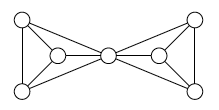
\includegraphics[width=0.35\textwidth]{figures/l08/ve-numbers.png}
  \end{center}
  For this particular example, we have
  \[
    \beta'(G) = 4 \qquad \alpha'(G) = 3 \qquad \beta(G) = 5 \qquad \alpha(G) = 2
  \]
\end{nexample}
\end{figure}

\subsection{K\"onig's Theorem}

\begin{theorem}[K\"onig, 1931]
  The maximum number of vertices of a matching in a bipartite
  graph \(G\) is equal to the minimum number of vertices of a
  vertex cover of its edges.
\end{theorem}

\begin{proof}
  Skipped (for now).
\end{proof}

\begin{remark}
  This theorem can also be restated as \textit{if \(G\) is a partite graph, then
  \(\alpha'(G) = \beta(G)\)}.
\end{remark}

\begin{figure}[ht]
\begin{nexample}
  Consider the following bipartite graph.
  \begin{center}
    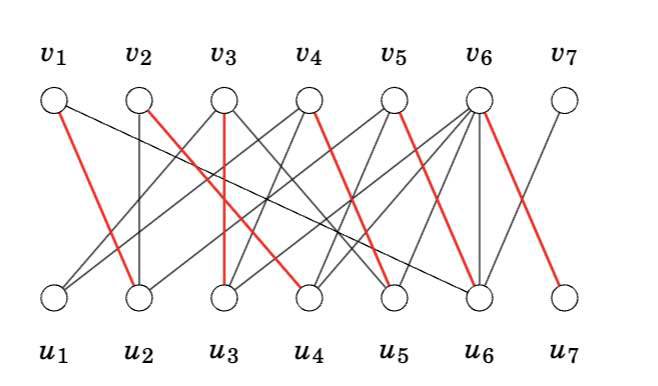
\includegraphics[width=0.5\textwidth]{figures/l08/matching-vertex-1}
  \end{center}
  We can see that this graph has the vertex cover
  \[ \{v_2, v_2, v_3, v_4, v_5, v_6\} \]
\end{nexample}
\end{figure}

\begin{figure}[ht]
\begin{nexample}
  Consider the following bipartite graph.
  \begin{center}
    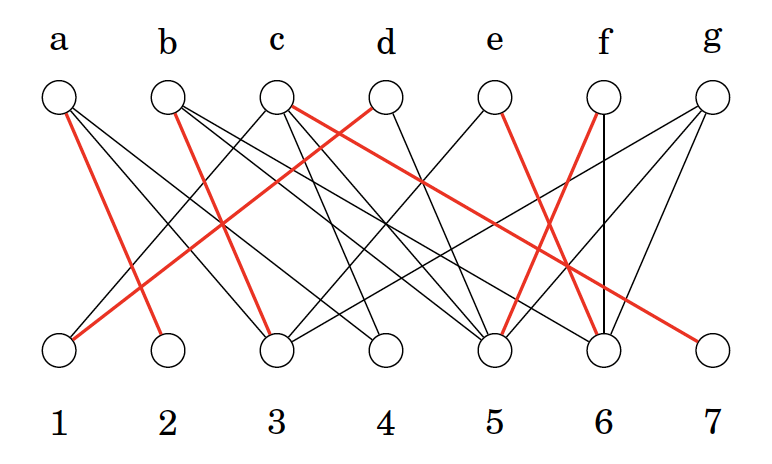
\includegraphics[width=0.5\textwidth]{figures/l08/matching-vertex-2}
  \end{center}
  We can see that this graph has the vertex cover
  \[ \{6, 3, 5, a, c, d\} \]
\end{nexample}
\end{figure}

\begin{theorem}
  Every \(r\)-regular bipartite graph with \(r \geq 1\) has a
  perfect matching.
\end{theorem}

\begin{proof}
  Let \(G\) be an \(r\)-regular bipartite graph where the vertices are split
  into sets \(A\) and \(B\). Note that \(|A| = |B|\). Consider \(\emptyset \neq S \subseteq A\).
  Suppose that \(|S| = k \geq 1\). It follows that the number of edges incident 
  to vertices in \(S\) is \(kr\). On the flip side, each vertex in \(N(S)\) is
  incident with at most \(r\) of the \(kr\) edges. Assume to the contrary that 
  \(|N(S)| = l < k\). Then, the maximum number of edges vertices in \(N(S)\) 
  can be incident to is \(lr < kr\). This is impossible. Hence, there must at
  least be \(k\) vertices in \(N(S)\) and thus, the marriage condition
  satisfies. Therefore, by Hall's Marriage Theorem, \(G\) has a perfect matching.
\end{proof}

\subsection{Gallai's Theorem}

\begin{theorem}[Gallai, 1959]
  For every graph \(G\) of order \(n\) containing no isolated vertices, we have
  \[ \alpha'(G) + \beta'(G) = n \]
\end{theorem}

\begin{proof}
  We will show this by showing that 
  \begin{equation}\label{eqn:gallai-proof-1}
    \alpha'(G) + \beta'(G) \leq n
  \end{equation}
  and 
  \begin{equation}\label{eqn:gallai-proof-2}
    \alpha'(G) + \beta'(G) \geq n
  \end{equation}

  We will first show \ref{eqn:gallai-proof-1}. Let \(k = \alpha'(G)\) be the
  size of the maximum matching. Notice that in this matching, there are
  \(k\) edges covering \(2k\) vertices. Then, we can use at most \(n-2k\) edges
  to cover the remaining \(n-2k\) vertices. So, the minimum number of edges in
  the edge cover \(\beta'(G) \leq (n-2k) + k = n-k\). Hence, we have that 
  \[ \alpha'(G) + \beta'(G) \leq k + (n-k) = n \]

